\documentclass[12pt,a4paper]{report}

\usepackage[utf8]{inputenc}
\usepackage[english]{babel}
\usepackage{amsmath}
\usepackage{amsfonts}
\usepackage{amssymb}
\usepackage{graphicx}
\usepackage{cite}
\usepackage{hyperref}
\usepackage[left=2cm,right=2cm,top=2cm,bottom=2cm]{geometry}

\author{Josep Puig}
\title{Session and Transport Layers}


\begin{document}
\maketitle


\chapter{Session and Transport Layer}

This layer is the one in charge of the free-of-error transference of data from one process to another. Therefore, its goal is to provide and guarantee a reliable and cheap flow of the data. 

Whereas the network layer oversees source-to-destination delivery of individual packets, it does not recognize any relationship between those packets. It treats each one independently, as though each piece belonged to a separate message, whether or not it does. The transport layer, on the other hand, ensures that the whole message arrives intact and in order, overseeing both error control and flow control source-to-destination level. 

\paragraph{}

A transport layer can be either connectionless or connection-oriented. A connectionless transport layer treats each segment as an independent packet and delivers it to the transport layer at the destination machine. A connection-oriented transport layer makes a connection with the transport layer at the destination machine first before delivering the packets. After all the data is transferred, the connection is terminated.

In the transport layer, a message is normally divided into transmittable segments. A connectionless protocol, such as UDP, treats each segment separately. A connectionoriented protocol, such as TCP and SCTP, creates a relationship between the segments using sequence numbers.
\paragraph{}


The transport layer is responsible for process-to-process delivery, i.e, the delivery of a packet, part of a message, from one process to another. Two processes communicate in a client/server relationship. 

Regarding addressing, at the transport layer, it is necessary a transport layer address, called a port number, to choose among multiple processes running on the destination host. The destination port number is needed for delivery, whereas the source port number is needed for the reply. 

The addressing mechanism allows multiplexing and demultiplexing by the transport layer.
	

\section{User Datagram Protocol (UDP)}
The User Datagram Protocol (UDP) is a connectionless, unreliable transport protocol. The only new feature regarding IP is that it provides process-to-process communication instead of host-to-host communication, and performs a very limited error checking. It might seem a powerless protocol, but its main point is that is a very simple protocol using a minimum of overhead. Therefore, if a process wants to send a small message and no extremely reliability is required, UDP is a good choice. 

Nevertheless, regarding the aim of this project, it is unacceptable to use UDP, since reliability is a key factor and must be taken into account.

\section{Stream Control Transmission Protocol (SCTP)}
The Stream Control Transmission Protocol is a new reliable, message-oriented transport layer protocol. Nevertheless, it has been designed and implemented mostly for Internet applications, such as IUA or SIP. But precisely it does not fit the goal of this project. 

Therefore, as there is a better choice (which will be deeply and widely explained in the following section), this protocol will not be considered. 


\section{ Transmission Control Protocol (TCP)}
The Transmission Control Protocol is again a process-to-process protocol. Consequently it uses port numbers. The main difference with the UDP is that TCP is a connection-oriented protocol, which means that creates a virtual connection between two TCP's in order to send data. Moreover, TCP uses flow and error control mechanisms. It is then a more reliable protocol that UDP. It adds connection-oriented and reliability features to the services of IP.

This will be the protocol chosen for this project, so it will be explained in detail in this section. 

\subsection{TCP Services}
Process-to-process communication: Like UDP, TCP provides this type of communication, using port numbers. In the following image there are the main well-known port numbers used by TCP.

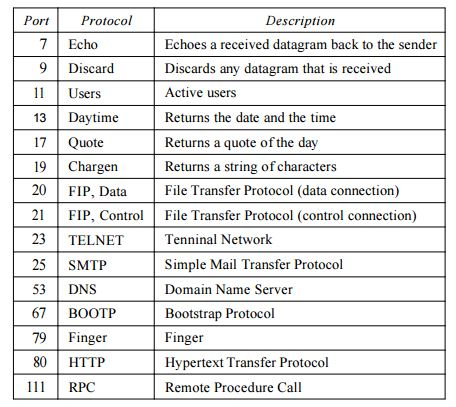
\includegraphics{TCP1}

\paragraph{}
Stream Delivery Service: as has been mentioned before, TCP, unlike UDP, is a stream-oriented protocol. UDP does not recognize any relationship between the datagrams. TCP, in contrast, allows the sending process to deliver data as a stream of bytes and allows the receiving process to obtain data as a stream of bytes. A way of explaining this would be an environment in which the two processes seems to be linked by and imaginary "tube" that carries the data across the Internet. The sending process produces the stream of bytes and the receiving process consumes them. This is, the first writes and the last reads. 

\paragraph{}
Sending and Receiving Buffers: Since the sending and receiving processes might not write or read data at the same speed, there is a need for storage in TCP. Therefore, TCP includes two buffers, the sending buffer and the receiving buffer. A deeper look into those buffers can be performed by looking at the bibliography. 

\paragraph{}
Full-Duplex Communication: TCP allows full-duplex service, so that data can flow in both directions at the same time. Each TCP has a sending and receiving buffer, and segments move in both directions. This feature is very important for the goal of this project.

\paragraph{}
Segments: Although buffering solves the problem of different speeds of producing and consuming, there is still one impotant feature to be discussed. The data needs to be sent in packets, not as a endless stream of bytes. Therefore, TCP groups a number of bytes together into a packet called a segment. A header is added to each segment for control purposes. 

\subsection{TCP features}
In order to provide the services that have been explained, TCP has some features that will be briefly discussed.


\subsubsection{Numbering Systems}
TCP keeps track of the segments being transmitted or received, using the header previoulsy discussed. 
There are in addition two fields, the sequence number and the acknowledgement number, which refer to the byte number, not the segment number.

TCP numbers all data bytes that are transmitted in a connection. Numbering is independent in each direction. When TCP receives bytes of data from a process, it stores them in the sending buffer and numbers them. Typically, it generates randomly a number between 0 and $2^{32}-1$ for the number of the first byte. For example, if the random number happens to be 1427 and the total data to be sent are 5000 bytes, the bytes are numbered from 1427 to 6426. This system is used for flow and error control.

After the bytes have been numbered, TCP assigns a sequence number to each segment that is being sent. The sequence number for each segment is the number of the first byte carried in that segment. This is, the value in the sequence number field of a segment defines the number of the first data byte contained in that segment. 

The value of the acknowledgement field in a segment defines the number of the next byte a party expects to receive. It is a cumulative number. 

\subsubsection{Flow Control}
TCP provides flow control, which means that the receiver can control the amount of data that if to be sent by the sender. The purpose of this is to avoid over-whelmed receivers. 

\subsubsection{Error Control}
In order to provide a reliable service, TCP implements an error control mechanism. It considers a segment as the unit of data for error detecting, even though there is also a byte-oriented control mechanism. 

\subsubsection{Congestion Control}
TCP also takes into account congestion in the network, by the detenning of the flow depending on the level of congestion in the network.





\subsection{Segment}
As has been explained before, a packet in TCP is called a segment. The aim of this point is to explain in detail what a segment is and how its structure is.

The typical format of the segment is shown in the next figure. 


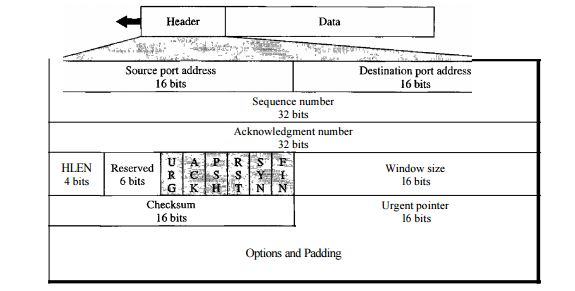
\includegraphics{TCP2}

The segment consists of a 20 to 60-byte header, followed by data frim the application program. The byte is 20-byte long if there are no options, and up to 60-bytes if there are options. 

The main parts of the format are to be discussed in the following lines.

\subsubsection{Source Port Adress}
This is a 16-bit field that states the port number of the application program in the host that is sending the segment. 

\subsubsection{Destination Port Adress}
It is also a 16-bit that defines the port number of the application program in the host that is receiving the segment. 

\subsubsection{Sequence Number}
This 32-bit field defines the number assigned to the first byte of the data contained in the segment considered. This numeration has been previously explained.

\subsubsection{Acknowledgement Number}
This is a 32-bit field that defines the byte number that the receiver of the segment is expecting to receive from the other party. If the receiver of the segment has successfully received byte number x, it defines x + I as the acknowledgement number. 

\subsubsection{Header Length}
A 4-bit field that indicates the number of 4-byte words in the TCP header. As seen, the length of the header can be between 20 and 60 bytes. Then, the value of this field can be between 5 and 15 (since $5\times	4=20$, and $15\times	4=60$). 

\subsubsection{Reserved}
This is a 6-bit field reserved for future usage.

\subsubsection{Control}
This field defines 6 different control bits or flags. One or more of those bits can be set at a time. 

\subsubsection{Window Size}
This fiels defines the size of the window, in bytes, that the other party must maintain. Since the length of this field is 16 bits, the maximum size of the windows is $2^{16}=65535$ bytes.  

\subsubsection{Urgent Pointer}
Another 16-bit field, which is only valid if the urgent flag is set, which means that the segment contains urgent data. In actually defines the number that must be added to the sequence number to obtain the number of the last urgent byte in the data section of the segment. 

\subsubsection{Options}
As has been explained, there can be up to 40 bytes of optional information in the TCP Header. This is the purpose of this last field. 


\section{Choice of protocol for the transport layer}
Three protocols have been discussed, the UDP, the SCTP and the TCP. The first one has some disadvantages which make it not suitable for the purpose of the project, such as the fact that no reliabililty is guaranteed, for example, amongst others. The second one is designed mostly for Internet applications, which does not fit the goals of this project. Therefore, the only candidate suitable for the project is the TCP, Transmission Control Protocol, which has already been widely explained and analyzed. As it has the required features that the project demands, it is the chosen protocol for this layer. 

\end{document}
